%%%%%%
%
% $Author: Abishek $
% $Date: 06.01.2025 $
% $Path: ML24-02-Gait-Pattern-Recognition\report\Contents\en$
% $Version: 1.0 $
% $Reviewed by: Abishek $
%
% !TeX encoding = utf8
% !TeX root = Rename
% !TeX TXS-program:bibliography = txs:///bibtex
%
%%%%%%

\chapter{Monitoring}

\section{Idea}
The objective of this project is to develop a self-contained gait analysis system using the Arduino Nano 33 BLE Sense. The device runs a CNN model locally to classify gait patterns as either normal or Parkinsonian, displaying results via an RGB LED. Since the system operates entirely offline, data retrieval and model updates are handled using Bluetooth Low Energy (BLE).

\begin{itemize}
	\item The user can export gait data using the nRF Connect app and upload it via a cloud link for further analysis.\cite{nordic2021nrfconnect}
	\item Model improvements are deployed remotely via BLE Over-the-Air (OTA) updates, ensuring continuous system enhancement without requiring internet access.\cite{nordic2021ota}
\end{itemize}

\section{Plan/Description}
The device logs gait data while providing immediate feedback through its LED indicators. Users are not required to perform monitoring themselves, as the system is designed to function autonomously. Periodically, the data is extracted via BLE, analyzed for improvements, and used to update the model.

\begin{itemize}
	\item BLE data extraction is conducted via nRF Connect, allowing users to upload exported files to a cloud service like Google Drive or Dropbox.
	\item Firmware updates containing improved CNN models are provided as downloadable files, which users install via nRF Toolbox DFU for BLE-based firmware updates.
\end{itemize}

\section{Getting New Data}
The system collects stride length, stride velocity, and step time data while the user walks. These values are stored on the device and retrieved via BLE when needed.

\begin{itemize}
	\item Users connect to the device using nRF Connect, export the recorded gait data, and upload it to a shared cloud link for analysis.
	\item This dataset is expanded with each new upload, allowing continuous learning and model refinement.
\end{itemize}


\section{Data Updating in the ML Pipeline}
Once new data is collected, it is processed and integrated into the existing machine learning pipeline to improve gait classification accuracy. The process includes preprocessing, retraining, validation, and deployment.

\begin{itemize}
	\item Raw data is cleaned, normalized, and merged with previously collected data before retraining the CNN model.
	\item The improved model is validated against the old version, ensuring an increase in accuracy before it is packed as a firmware update.
\end{itemize}
	\begin{figure}[h]

	\centering
	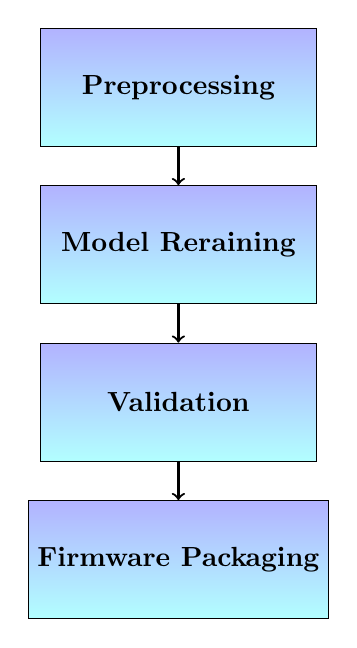
\begin{tikzpicture}[node distance=2cm, auto]
		
		% Define custom box style with gradient fill
		\tikzstyle{process} = [rectangle, draw, minimum width=3.5cm, minimum height=1.5cm, 
		text centered, font=\bfseries, 
		top color=blue!30, bottom color=cyan!30]
		
		% Nodes arranged in vertical order
		\node[process] (preprocess) {Preprocessing};
		\node[process, below of=preprocess] (train) {Model Reraining};
		\node[process, below of=train] (validate) {Validation};
		\node[process, below of=validate] (package) {Firmware Packaging};
		
		% Arrows
		\draw[->, thick] (preprocess) -- (train);
		\draw[->, thick] (train) -- (validate);
		\draw[->, thick] (validate) -- (package);
		
	\end{tikzpicture}
	


\caption{Data updation in ML pipeline}
\label{fig:pipeline update}
\end{figure}
\section{Checks}
To maintain system integrity, several checks are performed before deploying model updates or applying firmware changes. This ensures both data accuracy and device compatibility.

\begin{itemize}
	\item The new model undergoes validation testing to confirm it outperforms the previous version before deployment.
	\item Firmware compatibility checks ensure that the updated model can run efficiently within the memory constraints of the Arduino Nano BLE Sense.
\end{itemize}

\section{Code: Functions}
The Arduino Nano BLE Sense transmits gait data over BLE using a custom BLE service. The following function allows the device to advertise and send gait parameters:
\begin{lstlisting}[language=C++, caption=BLE Service Implementation for Gait Data Transmission in Arduino Nano BLE Sense]
	#include <ArduinoBLE.h>
	
	BLEService gaitService("180F");
	BLECharacteristic gaitDataCharacteristic("2A19", BLERead | BLENotify, 20);
	
	void setup() {
		Serial.begin(9600);
		BLE.begin();
		BLE.setLocalName("Gait Analyzer");
		BLE.setAdvertisedService(gaitService);
		
		gaitService.addCharacteristic(gaitDataCharacteristic);
		BLE.addService(gaitService);
		BLE.advertise();
		Serial.println("BLE Gait Analyzer Started");
	}
	
	void loop() {
		BLEDevice central = BLE.central();
		if (central) {
			float strideLength = 110.5;
			float strideVelocity = 90.2;
			int gaitType = 1; // 0 = Normal, 1 = Parkinsonian
			
			String gaitData = String(strideLength) + "," + String(strideVelocity) + "," + String(gaitType);
			gaitDataCharacteristic.writeValue(gaitData.c_str());
			
			delay(1000);
		}
	\end{lstlisting}

\begin{itemize}
	\item The BLE service transmits gait data for monitoring via nRF Connect on a smartphone.
	\item This function ensures that users can retrieve data in real-time, which can later be used for further analysis and improvements.
\end{itemize}

\section{Code: Test}
Testing ensures that BLE-based data transfer and firmware updates function correctly before deployment. The test includes validating BLE communication and verifying firmware installation.

\begin{itemize}
	\item Users can connect to the device via nRF Connect, view live gait data, and ensure logs are being transmitted correctly.
	\item Firmware updates are tested using nRF Toolbox DFU, confirming that the device successfully installs and runs the updated CNN model.
\end{itemize}

\section{Privacy}
All collected data remains stored locally on the device and is retrieved only when the user exports it. No automatic transmission to external servers occurs, ensuring user control over their data.

\begin{itemize}
	\item The BLE service is configured for read-only access, preventing unauthorized modifications to the device or data.
	\item Users manually upload exported logs to a secure cloud link, ensuring that they remain in control of when and where their data is shared.
\end{itemize}
\section{Robustness}
The system is designed to function reliably under real-world conditions, ensuring offline usability and secure data retrieval. BLE communication is structured to minimize disruptions, and updates are thoroughly tested before release.

\begin{itemize}
	\item The CNN model runs entirely on the device, ensuring continuous operation without requiring an internet connection.
	\item If a BLE connection fails, the system allows reconnection attempts without affecting stored data, making it resistant to interruptions.
\end{itemize}

\section{Process}
The full end-to-end process ensures seamless data collection, model improvement, and remote updates. Users follow simple steps to extract data and update the system when needed.

The device records gait data and provides real-time feedback via RGB LED. Users retrieve stored gait logs using BLE and upload them to a cloud link for analysis. The research team integrates new data into the machine learning pipeline and retrains the model. Once validated, the updated model is packaged as a firmware update and made available to users. Users install the update wirelessly using BLE, ensuring continuous improvement without internet access.

This structured approach ensures that the device remains accurate, up-to-date, and fully functional without requiring in-person servicing or customer intervention beyond simple BLE-based updates.
\begin{figure}[h]
	
	\centering

		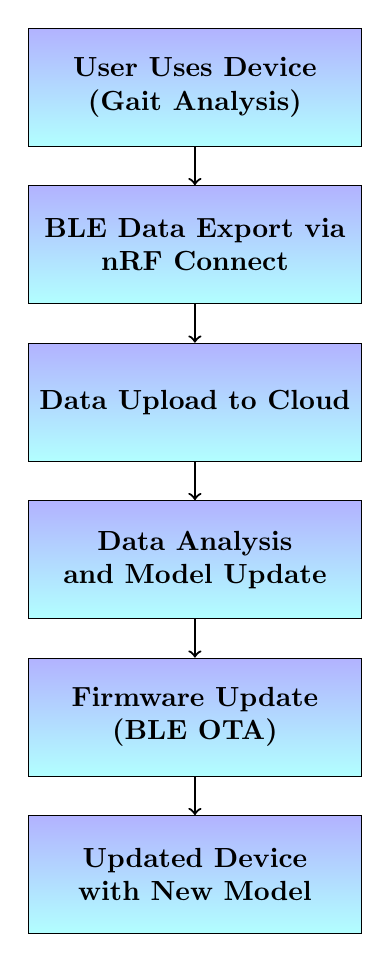
\begin{tikzpicture}[node distance=2.0cm, auto]
			
			% Define custom style for boxes with gradient fill
			\tikzstyle{process} = [rectangle, draw, text width=4cm, align=center, minimum height=1.5cm, 
			top color=blue!30, bottom color=cyan!30, font=\bfseries]
			
			% Nodes arranged in vertical flow
			\node[process] (user) {User Uses Device \\ (Gait Analysis)};
			\node[process, below of=user] (nrfconnect) {BLE Data Export via \\ nRF Connect};
			\node[process, below of=nrfconnect] (upload) {Data Upload to Cloud};
			\node[process, below of=upload] (analyze) {Data Analysis \\ and Model Update};
			\node[process, below of=analyze] (firmware) {Firmware Update \\ (BLE OTA)};
			\node[process, below of=firmware] (device) {Updated Device \\ with New Model};
			
			% Arrows connecting the boxes
			\draw[->, thick] (user) -- (nrfconnect);
			\draw[->, thick] (nrfconnect) -- (upload);
			\draw[->, thick] (upload) -- (analyze);
			\draw[->, thick] (analyze) -- (firmware);
			\draw[->, thick] (firmware) -- (device);
			
		\end{tikzpicture}





\caption{Workflow Diagram (High-level Process)}
\label{fig:Monitoring}
\end{figure}
